\subsection{Arduino-Plattform}\label{ss:Arduino}

Arduino ist ein Unternehmen, das all seine Produkte in enger Zusammenarbeit mit zugehörigen Community entworfen hat. Alle Entwicklungen basieren auf den Ideen und Konzepten, die die Gemeinschaft um das Unternehmen entwickelt hat. 

\begin{figure}[H] 
	\centering
	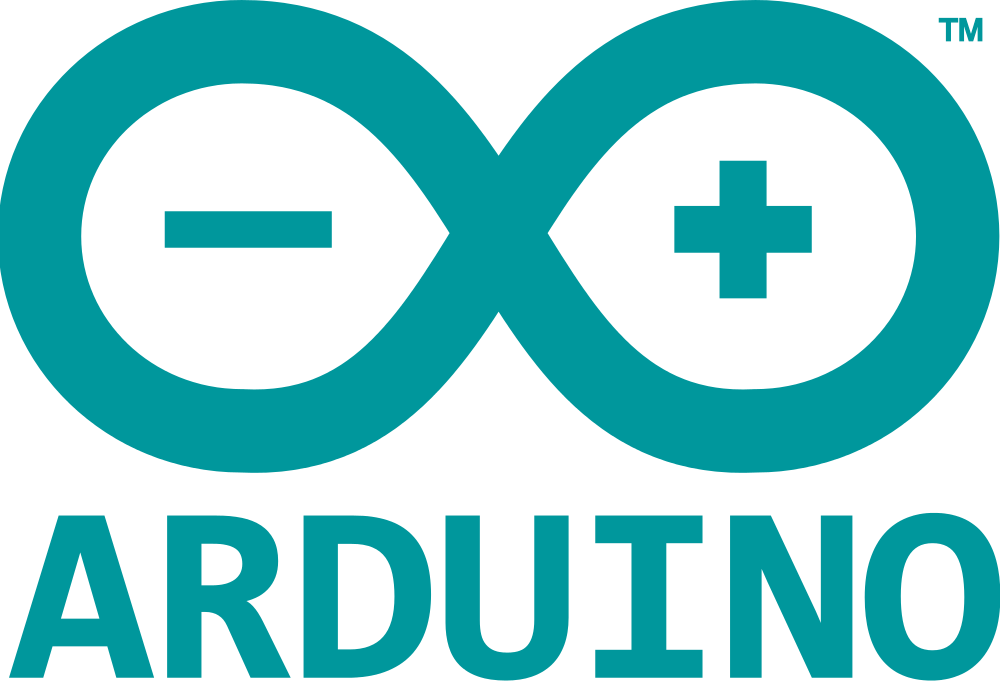
\includegraphics[scale=0.2]{Bilder/arduino}
	\caption{Das Arduino-Logo\cite{i:arduino}}
	\label{f:arduino}
\end{figure}

Das Unternehmen entwickelt Mikrokontrollerplatinen, die ihre Umwelt durch Sensoren wahrnehmen und auf äußere Einflüsse reagieren können. Alle Produkte sind vorgefertigt oder als Selbstbau-Kit erhältlich. Da die Baupläne aller Platinen durch Arduino quelloffen im Internet erhältlich sind, können die Produkte auch von Grund auf nachentworfen werden.\\

Das erste Arduino-Board, dass 2005 vorgestellt wurde, hat bereits viele Revisionen erhalten. In der aktuellsten Version ist es mit einem 16 \ac{MHz} 8-Bit Microcontroller ATmega328 der Firma Atmel bestückt. Es besitzt zusätzlich 32 Kilobyte Flash-Speicher von dem 0.5 Kilobyte durch den Bootloader belegt werden. Zur Ein- und Ausgabe, sowie zum Anschließen von Sensoren besitzt die Platine 14 digitale Input- oder Output-Pins, sowie 6 analoge input Pins und einen \ac{USB}-Anschluss. Betrieben wird die Platine mit einem 7-12V Netzteil \cite{ws:arduinouno}.
Die Platine wird von dem italienischen Unternehmen SmartProjects produziert, ist jedoch aufgrund des quelloffenen Platinenplans auch selbst zusammensetzbar.\\

\begin{figure}[H] 
	\centering
	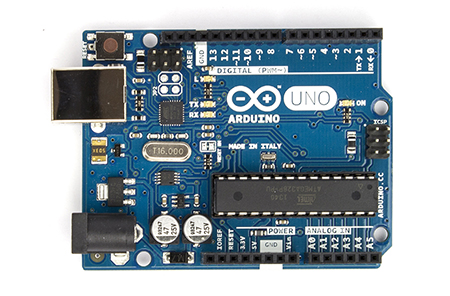
\includegraphics[scale=0.6]{Bilder/arduinouno}
	\caption{Die Front der dritten Arduino Uno Revision\cite{i:arduinouno}}
	\label{f:arduinouno}
\end{figure}

Die Arduino-Plattform besitzt eine eigene \ac{IDE}, in der die Software für den Microcontroller entwickelt werden kann. Der Mikrocontroller wird mit einer stark vereinfachten Form der Programmiersprachen C und C++ angesprochen. Insbesondere technische Informationen wie Header-Files werden vor dem Programmierer verborgen. Für Anfänger bietet die \ac{IDE} mehrere Einstiegshilfen, die das Programmieren erleichtern.\\
Ein Beispiel für die Einstiegshilfen sind die strukturgebenden Funktionen setup(), sowie loop(). Während in der Setup-Methode alle Aktionen definiert werden müssen, die beim Programmstart durchgeführt werden sollen, wird der Code in der Loop-Methode unbegrenzt oft wiederholt.
Ein Beispielcode, der eine an Pin 13 angeschlossene LED blinken lässt, lautet wie folgt:\\

\begin{lstlisting}[language=c,caption={Simpler Arduino-Code, der eine LED blinken lässt},label=lst:blink,frame=single] 
int led = 13; //LED an Pin 13

void setup() {                
	pinMode(led, OUTPUT);     
}

void loop() {
	digitalWrite(led, HIGH);  
	delay(1000);               
	digitalWrite(led, LOW);   
	delay(1000);               
}
\end{lstlisting}

\vspace{1cm}

Seit der Entwicklung der Arduino-Boards erfreuen sich diese großer Beliebtheit. So wurden bis 2013 insgesamt 700.000 zusammengesetzte Platinen verkauft\cite{ws:sellnumb}.\\

Viele der Projekte, die mit Arduino-Platinen durchgeführt werden, beinhalten Benutzerinteraktion. Auch für Kunstinstallationen werden die Einplatinencomputer gerne verwendet\cite{ws:elektor}.
